\documentclass[fleqn,10pt]{article}

\usepackage[left=2cm,right=2cm,
top=1.25cm,
bottom=0.5cm,%
headheight=11pt,%
letterpaper]{geometry}



\usepackage[left=2cm,right=2cm,
			top=1.25cm,
			bottom=2.25cm,%
			headheight=11pt,%
			letterpaper]{geometry}
			

\frenchspacing			

\nonstopmode



\usepackage{lmodern}
\usepackage[T1]{fontenc}
\usepackage[utf8]{inputenc}

%\usepackage[sfdefault]{roboto}
\usepackage[sfdefault,light]{roboto}


\usepackage{noweb}

\usepackage{multicol}
\usepackage{fancyhdr}
\usepackage{blindtext,graphicx}
\usepackage[absolute]{textpos}
%\usepackage[parfill]{parskip}
\usepackage{parskip}
\setlength{\parskip}{\baselineskip}

\usepackage[colorlinks=true,urlcolor=blue,citecolor=brown, urlbordercolor=black]{hyperref}


\makeatletter
\Hy@AtBeginDocument{%
	\def\@pdfborder{0 0 1}% Overrides border definition set with colorlinks=true
	\def\@pdfborderstyle{/S/U/W 0.5}% Overrides border style set with colorlinks=true
	% Hyperlink border style will be underline of width 1pt
}
\makeatother

\usepackage{gensymb}
\usepackage{csquotes}
\usepackage{amsmath}
\usepackage{fontawesome}
\usepackage{orcidlink}
\usepackage{standalone}
\usepackage{pdfpages}
\usepackage{subfiles}
\usepackage{svg}
\listfiles
\svgpath{{../biology/simulation/GROMACS/BUMPy_bilayer/data/}{../electronics/propagation/}}

\usepackage{sidecap}
\usepackage{float}
\usepackage{amssymb}
\usepackage{textcomp}
\usepackage{lettrine}

\usepackage{subfig}


\setlength{\footnotesep}{0.7\baselineskip}



% This allows the endnote and reference footnotes to float with the text.
%\usepackage{enotez}
%\let\footnote\endnote
%\let\footnotetext\endnotetext
%\let\footnotemark\endnotemark

\usepackage{soul} % strikethrough \st


%\usepackage{draftwatermark}
%\SetWatermarkText{DRAFT}
%\SetWatermarkScale{0.25}

\usepackage{booktabs,caption}
\usepackage[flushleft]{threeparttable}

%\usepackage{biblatex}
\usepackage[backend=bibtex8, sorting=none, style=phys]{biblatex}
% style=chem-angew
\let\cite\footfullcite



%\let\cite\footcite

\addbibresource{references.bib}
%biblatex has a zoterordfxml
% might avoid the need for python bibtex_collections.py



\usepackage{etoolbox}
\AtBeginEnvironment{quote}{\small}




\usepackage{pifont}
\newcommand{\cmark}{\ding{51}}%
\newcommand{\xmark}{\ding{55}}%


\newcommand{\wikinote}[1]{\textsuperscript{[\color{blue}{\textit{\textbf{#1}}}]}}
\newcommand{\citationneeded}[1][]{\textsuperscript{[\color{blue}{\it \bf{citation needed}#1}]}}
\newcommand{\dubiousdiscuss}[1][]{\textsuperscript{\color{blue} [{\it \bf{dubious-discuss}}]} }

\newcommand{\light}[1]{\textcolor{gray}{#1}}

\newcommand{\ntilde}{\char`~}

%
%
\usepackage{titlesec}
%
%% custom section


\titleformat{\section}
{\normalfont\LARGE\bfseries}{\thesection}{1em}{}
%\titleformat{\section}
%{\normalfont\LARGE\bfseries\PRLsep}
%{{{{\itshape \thesection\hskip 9pt\textpipe\hskip 9pt}}}}{0pt}{}

%% custom section
%\titleformat{\subsection}
%{\normalfont\Large\bfseries\PRLsep}
%{{{{\itshape \thesection\hskip 9pt\textpipe\hskip 9pt}}}}{0pt}{}
%
%
%


\newcommand{\Wsqm}{$\text{ W/m}^2$}

\newcommand{\ghfile}[1]{\href{https://github.com/0xDBFB7/covidinator/tree/master/#1}{\faGithub/\url{#1} }}

%\newcommand{\supercite}[1]{}
%\newcommand{\supercollect}[1]{}


\newlength{\PRLlen}
\newcommand*\PRLsep[1]{{\itshape \Large\settowidth{\PRLlen}{#1}\advance\PRLlen by -\textwidth\divide\PRLlen by -2\noindent\makebox[\the\PRLlen]{\resizebox{\the\PRLlen}{1pt}{$\blacktriangleleft$}}\raisebox{-.5ex}{#1}\makebox[\the\PRLlen]{\resizebox{\the\PRLlen}{1pt}{$\blacktriangleright$}}\bigskip}}


\renewcommand{\thefootnote}{\textcolor{blue}{[\arabic{footnote}]}}

\usepackage{multirow}



\usepackage{graphicx}
\graphicspath{ {../media/} 
				{../firmware/eppenwolf/runs/sic_susceptor/} 
				{../biology/simulation/GROMACS/BUMPy_bilayer/data/}
			}


\usepackage{tcolorbox}
\newtcolorbox{protocol}{colback=yellow!5!white,colframe=yellow!75!black}
\newtcolorbox{equipment}{colback=orange!5!white,colframe=orange!75!black}
\newtcolorbox{autem}{colback=red!5!white,colframe=red!75!black}
\newtcolorbox{toolchain}{colback=blue!5!white,colframe=blue!40!black!40}
\newtcolorbox{sidenote}{colback=cyan!5!white,colframe=blue!40!black!40}
%https://tex.stackexchange.com/questions/66154/how-to-construct-a-coloured-box-with-rounded-corners

%\usepackage[sfdefault,light]{roboto}

\setlength{\TPHorizModule}{1cm}
\setlength{\TPVertModule}{1cm}





%%%%********************************************************************
% fancy quotes
\definecolor{quotemark}{gray}{0.7}
\makeatletter
\def\fquote{%
	\@ifnextchar[{\fquote@i}{\fquote@i[]}%]
}%
\def\fquote@i[#1]{%
	\def\tempa{#1}%
	\@ifnextchar[{\fquote@ii}{\fquote@ii[]}%]
}%
\def\fquote@ii[#1]{%
	\def\tempb{#1}%
	\@ifnextchar[{\fquote@iii}{\fquote@iii[]}%]
}%
\def\fquote@iii[#1]{%
	\def\tempc{#1}%
	\vspace{1em}%
	\noindent%
	\begin{list}{}{%
			\setlength{\leftmargin}{0.05\textwidth}%
			\setlength{\rightmargin}{0.05\textwidth}%
		}%
		\item[]%
		\begin{picture}(0,0)%
		\put(-15,-5){\makebox(0,0){\scalebox{3}{\textcolor{quotemark}{``}}}}%
		\end{picture}%
		\begingroup\itshape}%
	%%%%********************************************************************
	\def\endfquote{%
		\endgroup\par%
		\makebox[0pt][l]{%
			\hspace{0.8\textwidth}%
			\begin{picture}(0,0)(0,0)%
			\put(15,15){\makebox(0,0){%
					\scalebox{3}{\color{quotemark}''}}}%
			\end{picture}}%
		\ifx\tempa\empty%
		\else%
		\ifx\tempc\empty%
		\hfill\rule{100pt}{0.5pt}\\\mbox{}\hfill\tempa,\ \emph{\tempb}%
		\else%
		\hfill\rule{100pt}{0.5pt}\\\mbox{}\hfill\tempa,\ \emph{\tempb},\ \tempc%
		\fi\fi\par%
		\vspace{0.5em}%
	\end{list}%
}%
\makeatother



\titlespacing{\section}{0pt}{\parskip}{0\parskip}
\titlespacing{\subsection}{0pt}{\parskip}{0\parskip}
\titlespacing{\subsubsection}{0pt}{\parskip}{0\parskip}






%%%%********************************************************************
%title link to doi
\newbibmacro{string+doiurlisbn}[1]{%
	\iffieldundef{doi}{%
		\iffieldundef{url}{%
			\iffieldundef{isbn}{%
				\iffieldundef{issn}{%
					#1%
				}{%
					\href{http://books.google.com/books?vid=ISSN\thefield{issn}}{#1}%
				}%
			}{%
				\href{http://books.google.com/books?vid=ISBN\thefield{isbn}}{#1}%
			}%
		}{%
			\href{\thefield{url}}{#1}%
		}%
	}{%
		\href{https://doi.org/\thefield{doi}}{#1}%
	}%
}

\DeclareFieldFormat{journaltitle}{\usebibmacro{string+doiurlisbn}{\mkbibemph{#1}}}



\begin{document}

%Daniel Correia\\
%30 Lamont Creek Drive\\
%Wasaga Beach, Ontario\\
%L9Z 1J9
%
%Canadian Light Source Inc.\\
%44 Innovation Boulevard\\
%Saskatoon, SK S7N 2V3\\
%Canada\\
%
%\noindent\par
%\noindent\makebox[\textwidth][c]{%
%\begin{minipage}{0.7\textwidth}
%Dear Recruiting Manager,\\
%
%Hello!\\
%
%In response to SXRMB Support Scientist position number 2021-2, kindly find my resume attached. \\
%
%I have about 5 years of experience founding and managing an electronics company and performing associated research, along with a B.Sc. in Science. \\\\ Skills particularly suited to the CLS include some experience in the design and fabrication of high vacuum systems, and with beam simulation codes such as IBSimu and Warp.\\
%
%I also have a small amount of recent experience in physical virology and applied microbiological technique that may be of some use.\\
%
%
%
%I am willing to relocate for this position, and am available for a remote interview at any time. \\\\
%
%Thanks for your time!
%\end{minipage}}
%%\newgeometry{textwidth=10cm,textheight=10cm}
%
%
%
%%\restoregeometry
%
%
%\clearpage

\begingroup
\fontseries{t}\selectfont

{\Huge Hi, I'm Daniel.}

\endgroup

\light{\large \textit{Science rules!}}



\small{{Daniel Correia}\ \orcidlink{0000-0002-9353-0216} | \href{https://github.com/0xDBFB7}{github.com/0xDBFB7} | therobotist@gmail.com ({\footnotesize preferred}) | dcorreia@safesump.com | @0xDBFB7 on Twitter
\light{\makebox[\linewidth]{\rule{\textwidth}{0.4pt}}}


\begin{multicols}{1}

\begin{tcolorbox}
\textbf{Education:\\}
B.Sc. in Science from York University, Physics stream. Graduated in the fall of 2021.
\end{tcolorbox}
%
\section*{SafeSump Inc.}

CEO/CTO of four-year project to design and produce a failure-resistant water pump system. Funded by a \$37,500 Ontario Centres of Excellence grant (2017-2020) followed by a \$75,000 government contract (2018-2020).

Broad overview of skills gained:

\begin{itemize}
	\item \textbf{Electronics}: Production electronics design and design-for-manufacturing; rapid prototyping of ultrasonic and capacitive sensors, among others
	\item \textbf{Software and firmware}: Version control. Frontend and backend server programming; Linux administration, programming of production utilities and scripts. Writing and maintaining a 30k SLOC codebase of C, Python and C++.
	\item \textbf{Soft skills}: Pair programming, time management, writing.
\end{itemize}


\section*{Viral electroporation}

A 10-month attempt to follow up experimentally on previous research regarding the dielectric properties of viruses, in the hopes of harnessing a phenomenon known as irreversible membrane electroporation, via optimized Brillouin precursors.

This required some literature review and a degree of care in experimental design, but also required several specialized pieces of equipment:

A custom, inexpensive synchronous photon-counting fluorescence system, allowing amplification-free quantification of dsDNA at sub-nanogram resolution.

Development of an inexpensive 12 GHz microwave absorption spectrometer (albeit unused in the final experiment)

Electromagnetic modelling of tissue and experimental system parameters via FDTD; sub-nanosecond kilovolt pulse generation; numerical optimization of dispersive pulses.

Data was collected on the model organism bacteriophage T4, necessitating wet-lab techniques.\\ \\ Due to several missteps in design on my part, however, the study was thoroughly inconclusive. A report on the same is due to be edited.


Broad overview of skills gained:
\begin{itemize}
	\item \textbf{Documentation}: LaTeX, Jupyter notebooks, Mathematica, Reference management
	\item \textbf{Software}: Data analysis and automation; Python, C++, and a smattering of many others
	\item \textbf{Simulation}: Several dozen toolchains were in use, ranging from modified open-source electromagnetic simulation systems to molecular dynamics with GROMACS.
	\item \textbf{Electronics}: Microwave electronics design, PCB design with KiCAD
	\item \textbf{Fabrication}: Electronics prototyping, CNC mill and lathe operation, micromachining, microfluidics
\end{itemize}


\section*{Vacuum systems}

A 2-year attempt to develop a high-current ion beam lithography system, involving the ion-beam simulation tools noted in the cover letter and several custom solvers.
	
\end{multicols}



\begin{figure}[H]
	\centering
	
	\subfloat[]{
		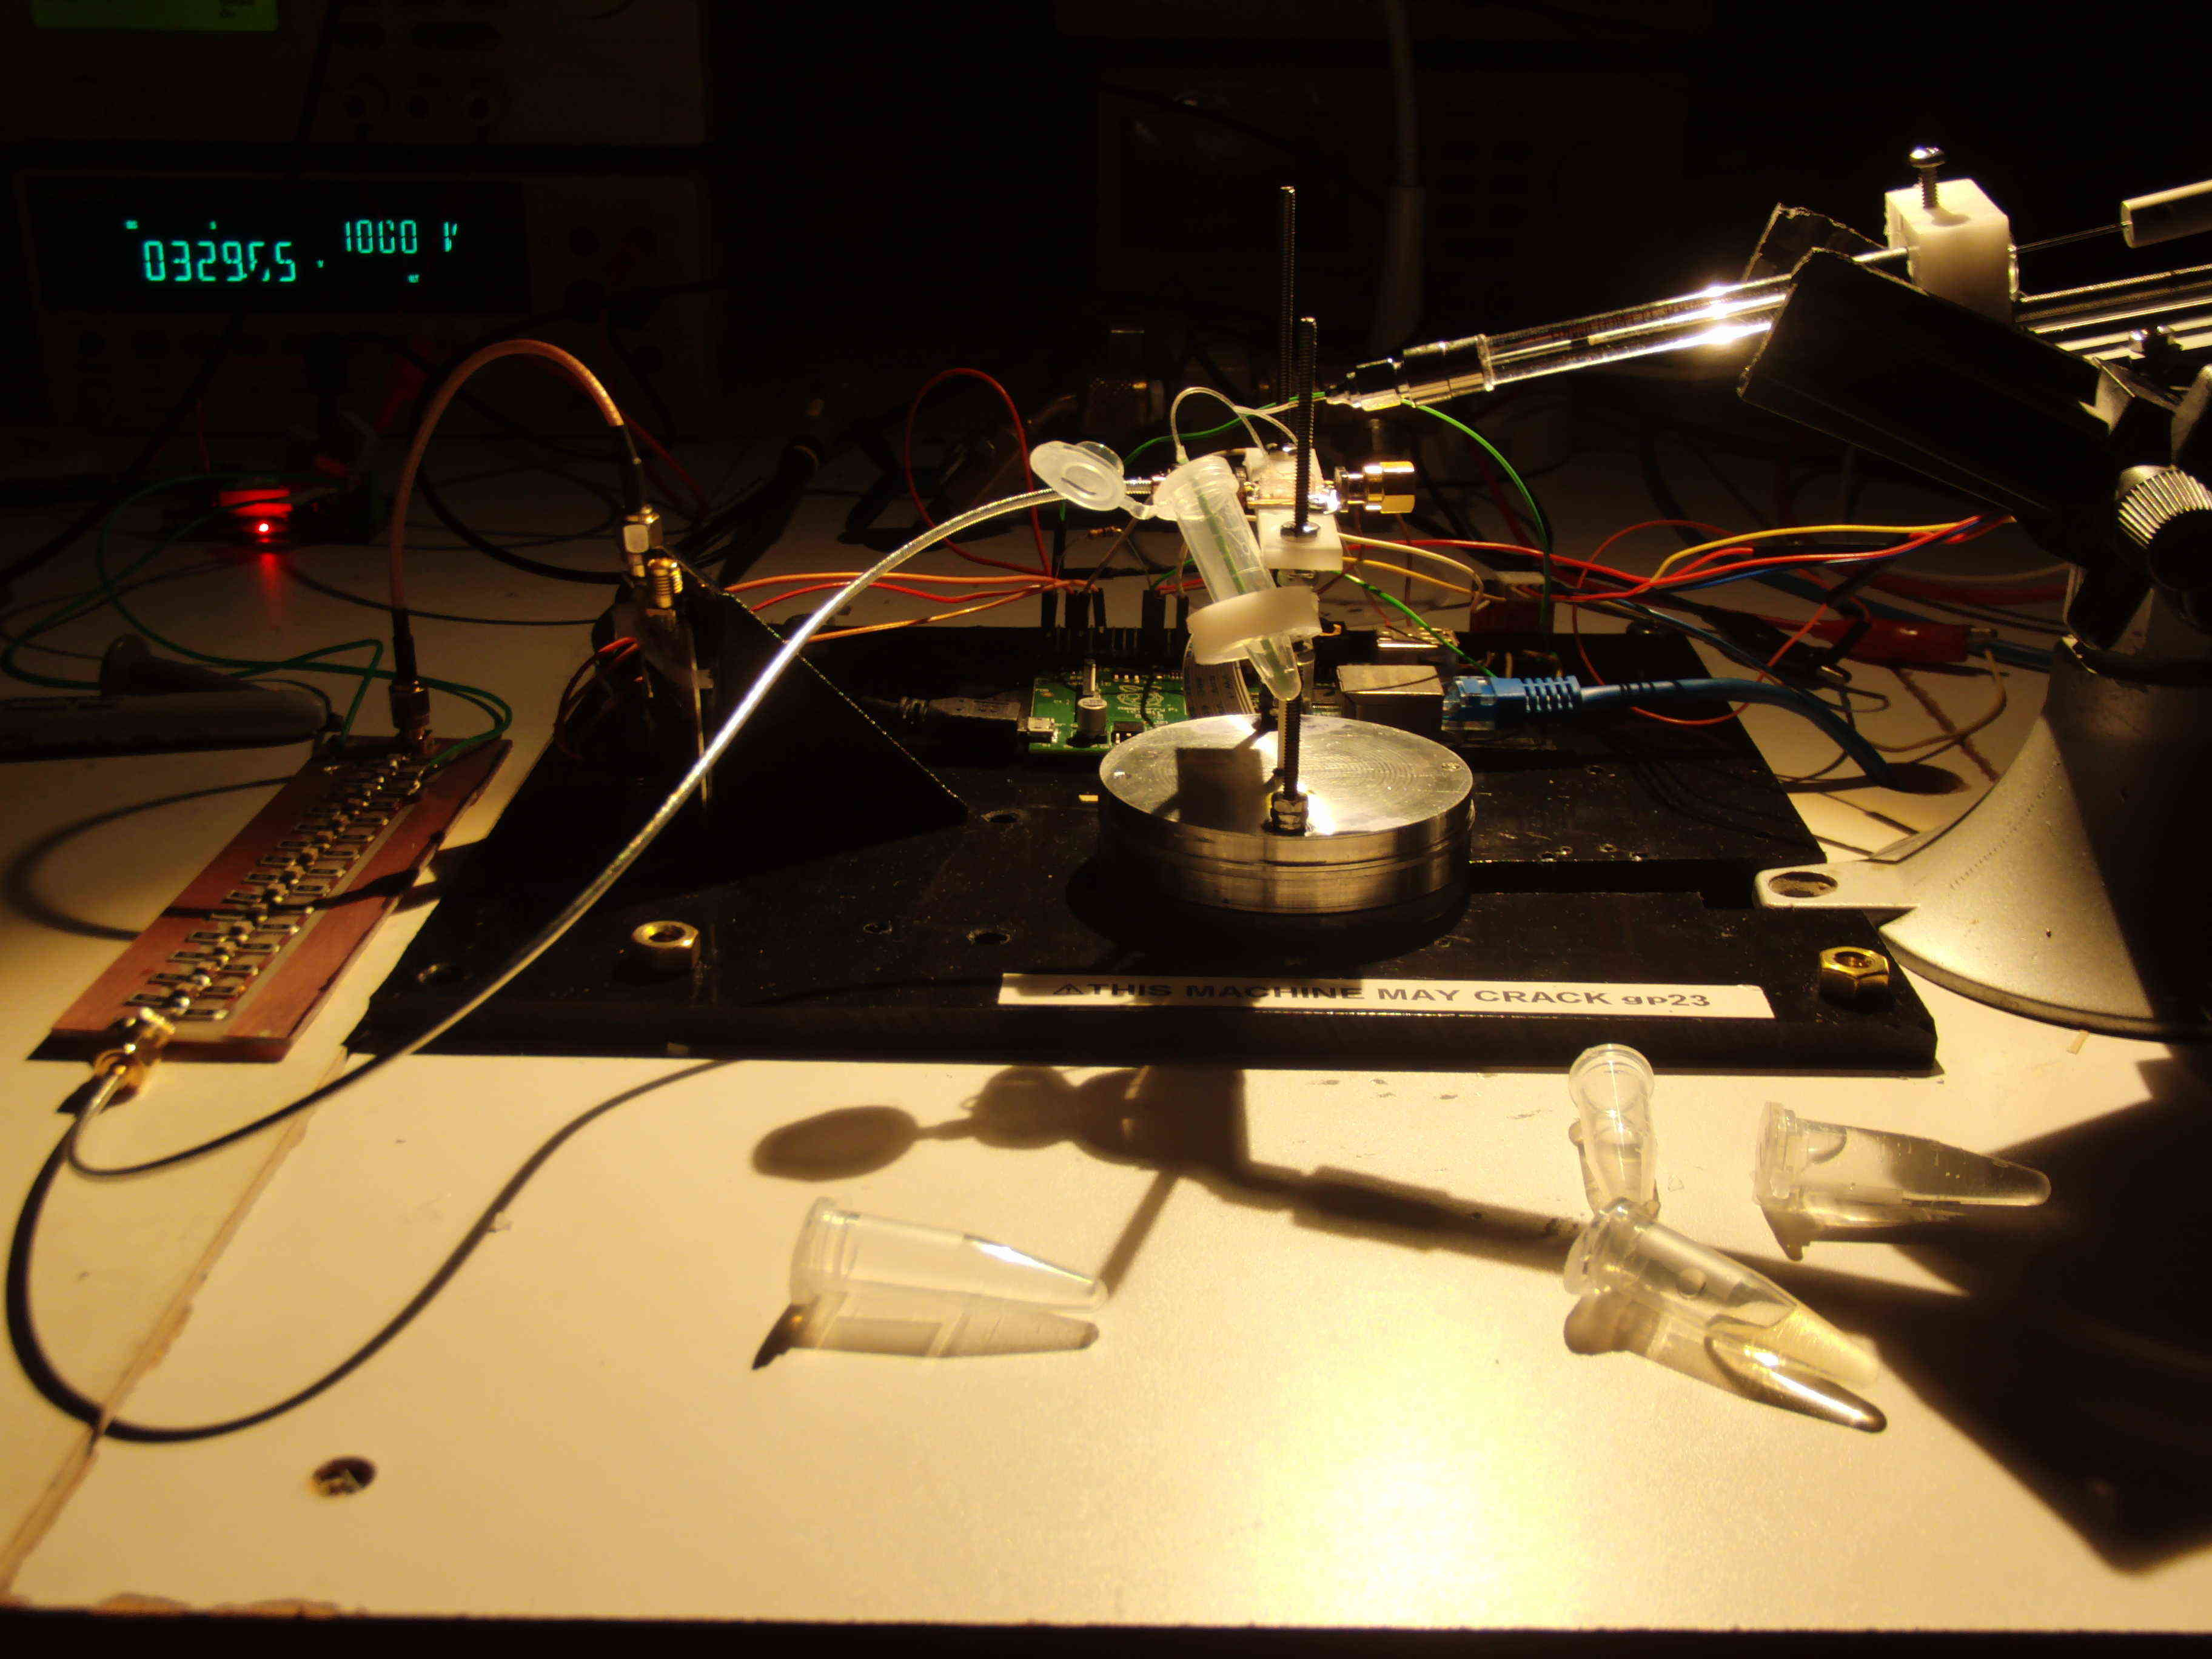
\includegraphics[width=0.5\textwidth]{pulse_exposure_setup}
		
	}
	\subfloat[]{
		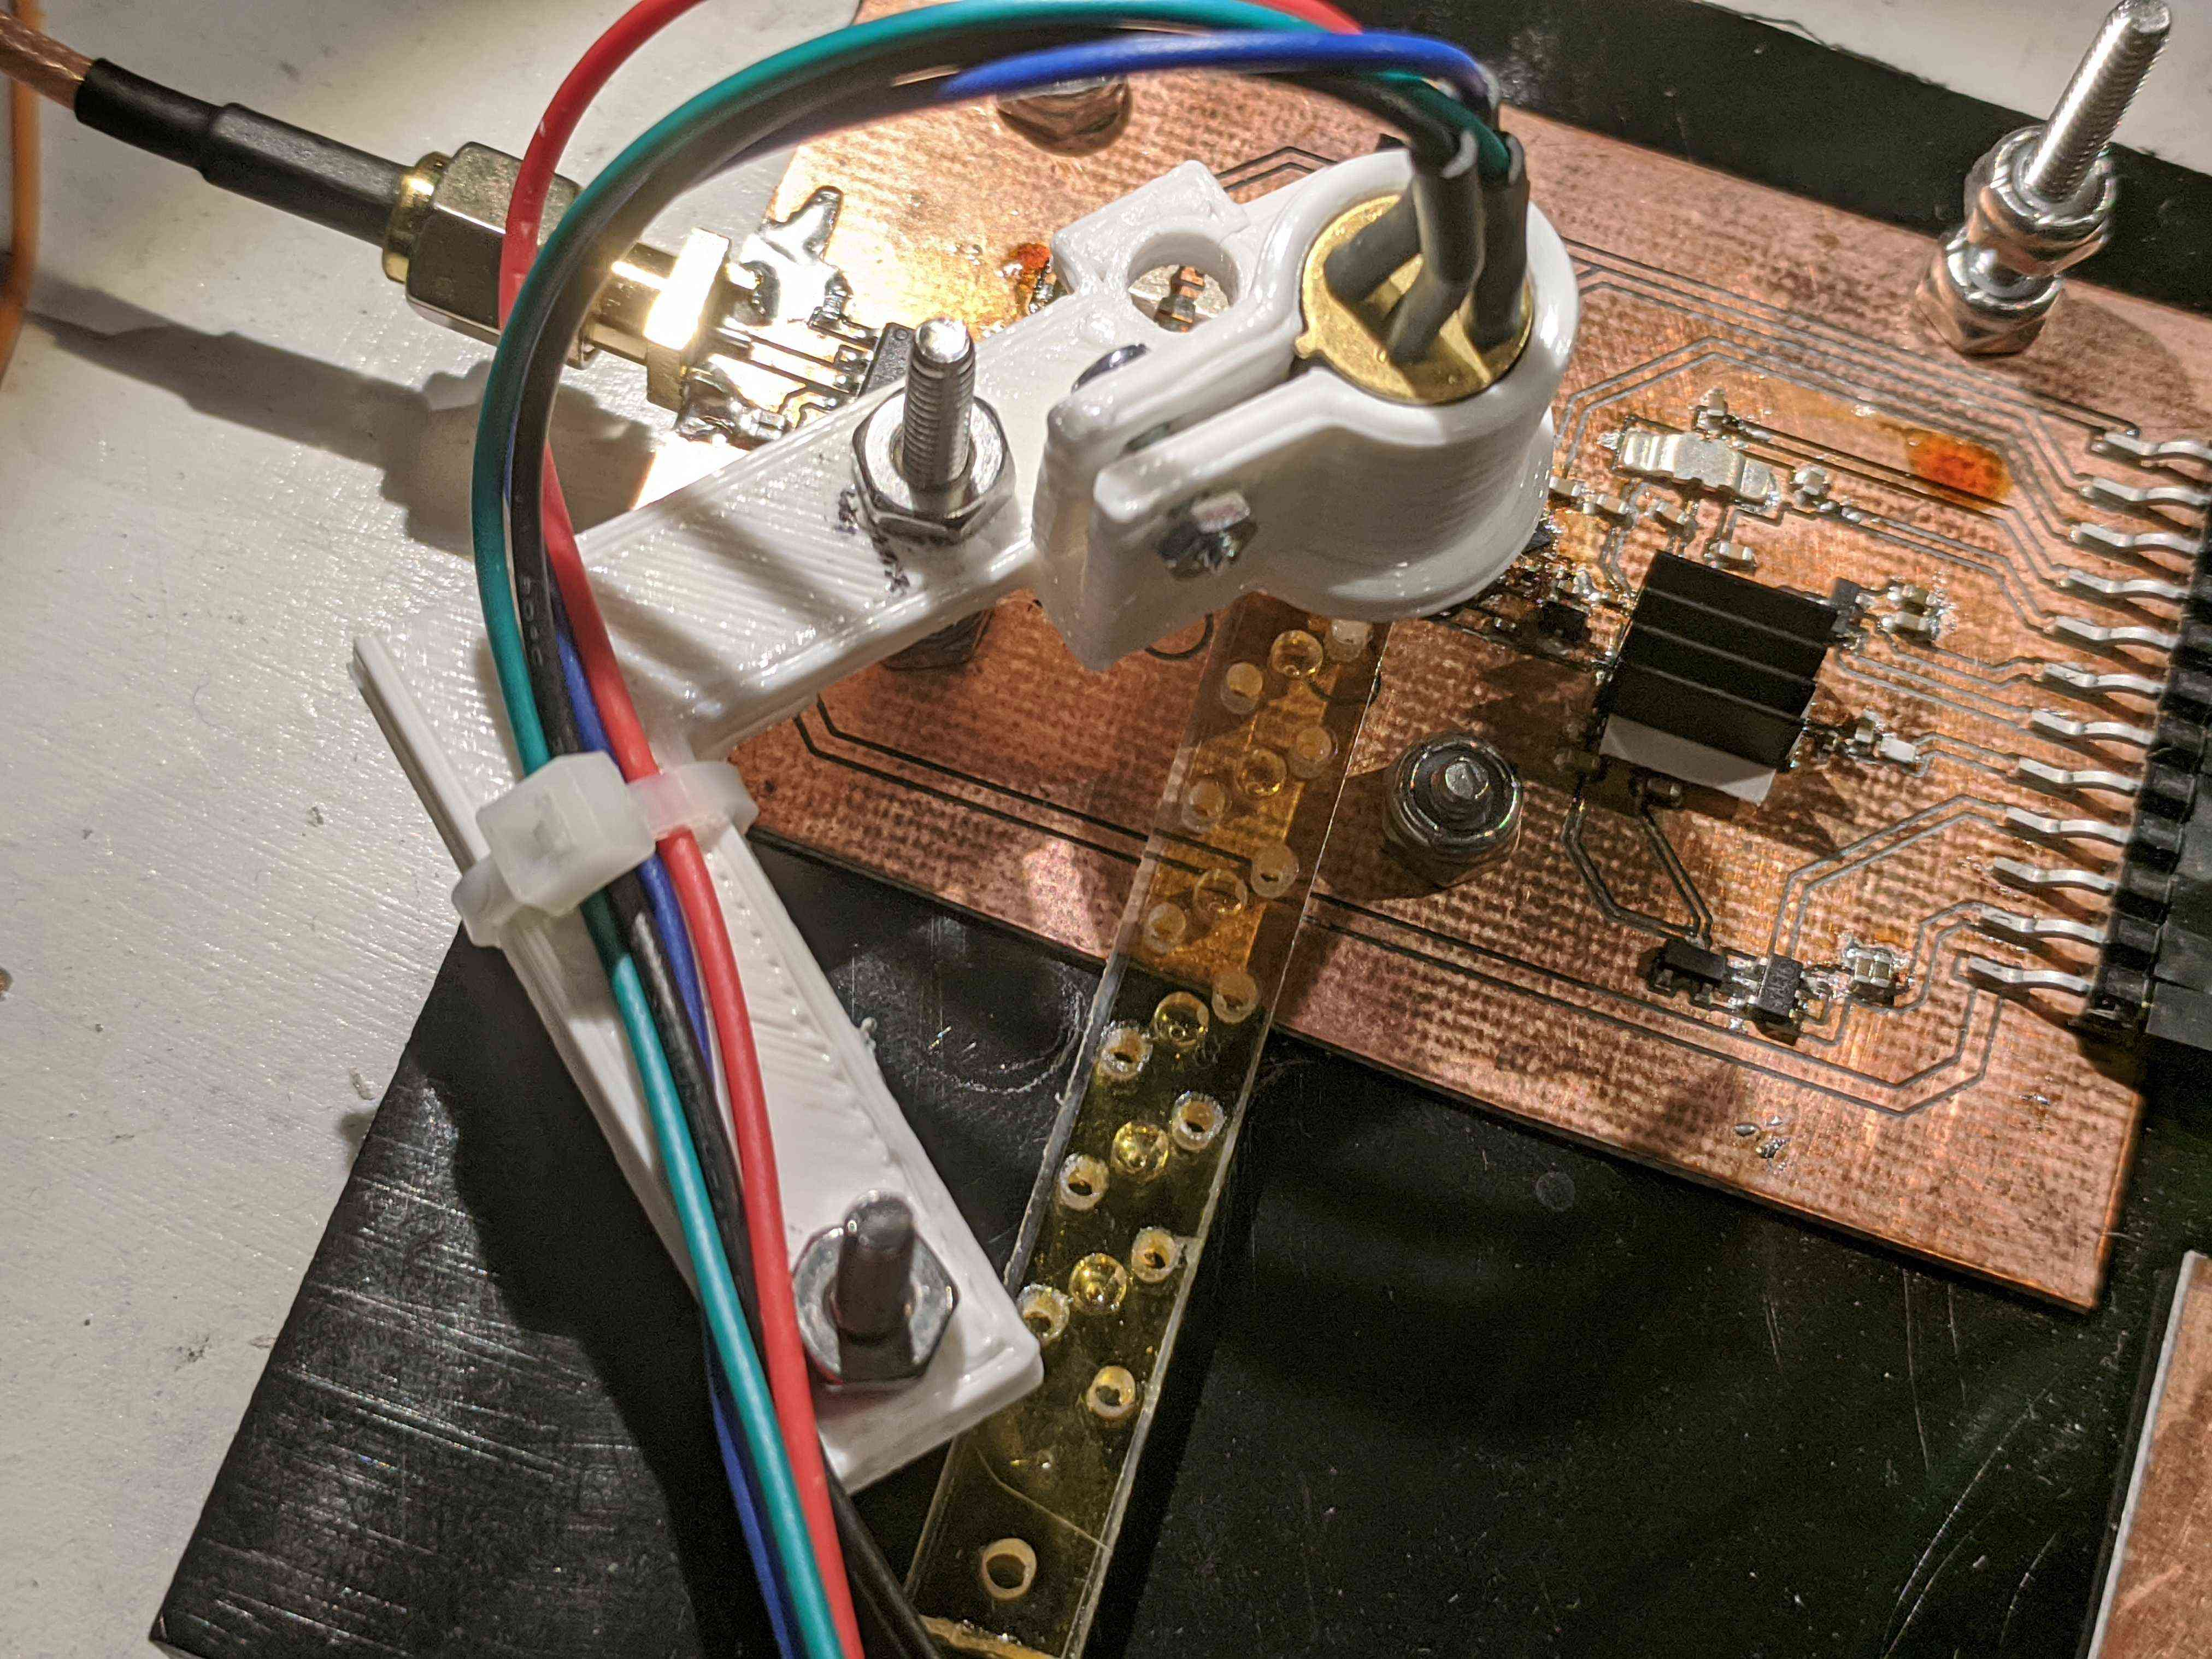
\includegraphics[width=0.5\textwidth]{eppenwolf_2}
	}
	
	\subfloat[]{
		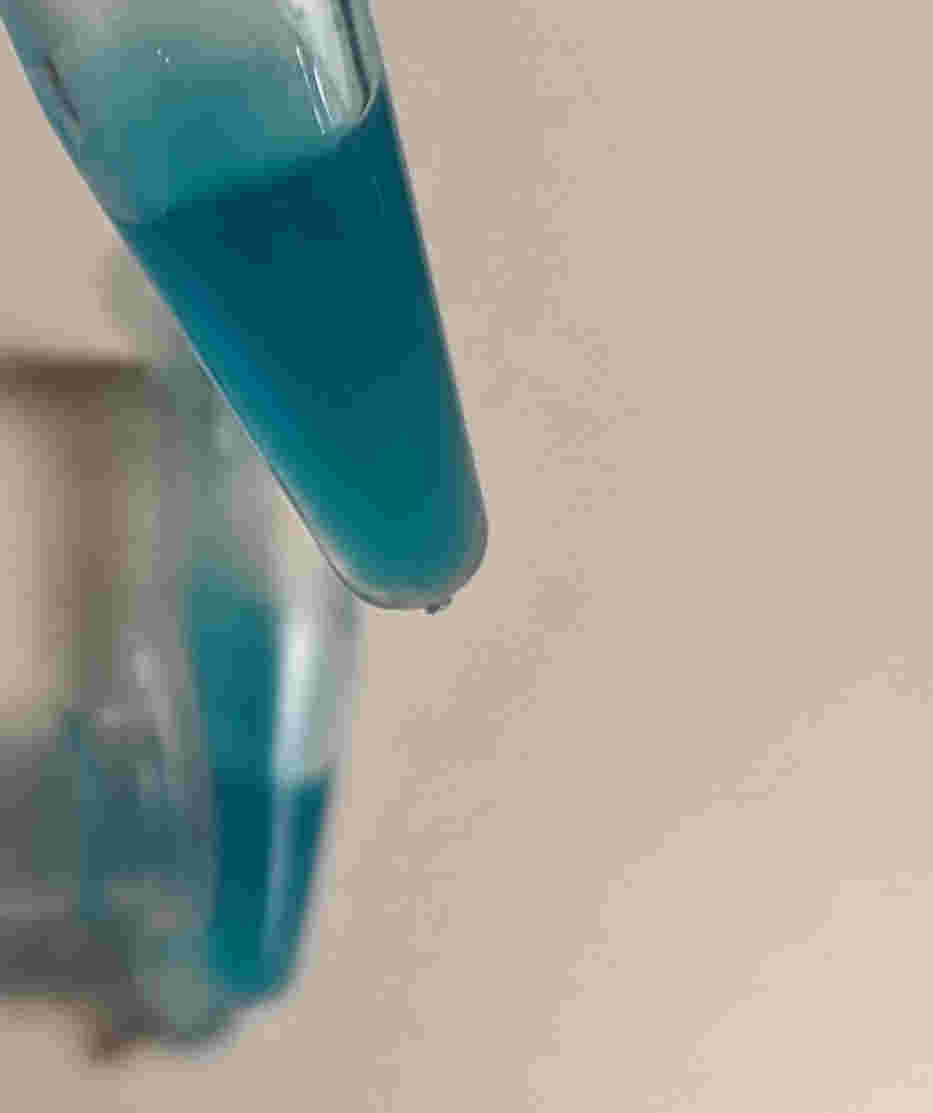
\includegraphics[width=0.4\textwidth]{x_gal.jpg}
	}
	\hfill
	\subfloat[]{
		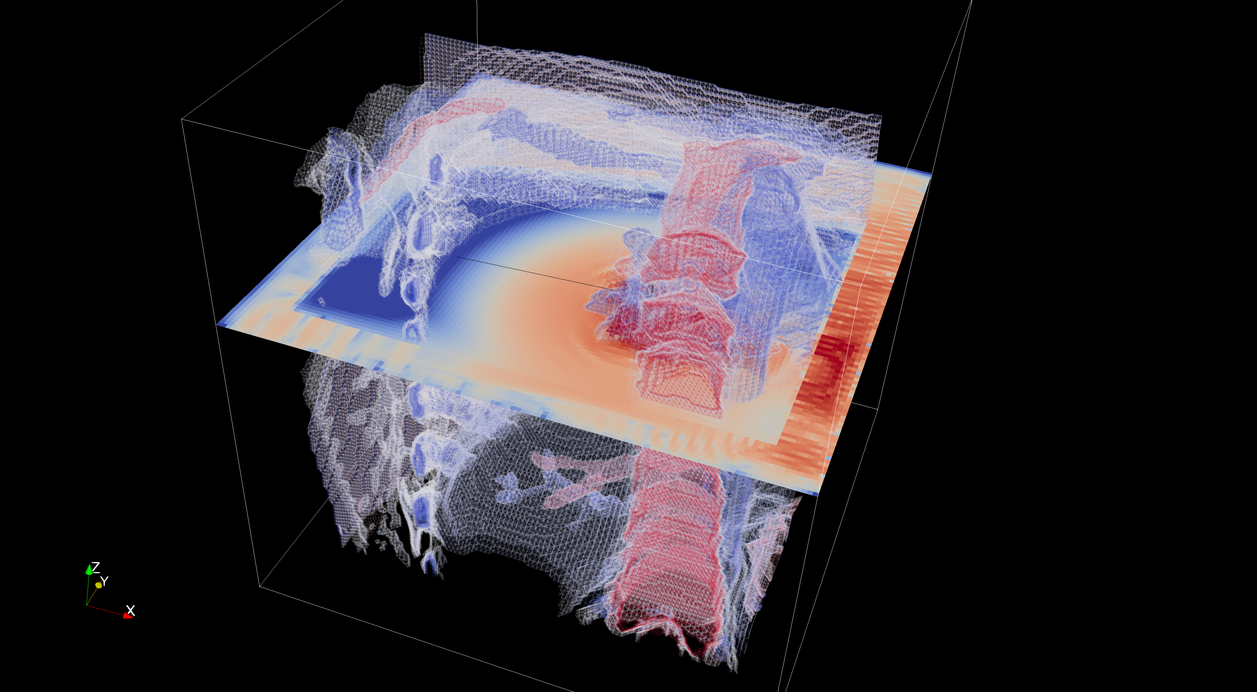
\includegraphics[width=0.5\textwidth]{bronch_9GHz_500W_2}
	}
	
	\caption*{\\ (a) The sub-nanosecond pulse generator and microfluidic exposure cell designed to induce electroporation. \\ (b) A 12 GHz microwave absorption spectrometer. \\(c) The very pretty opalescent blue culture caused by E. coli B trying to metabolize lactose in an indicator for the enzyme $\beta$-galactosidase.\\ (d) An FDTD simulation of electromagnetic interaction with tissue. }
\end{figure}




\begin{figure}[H]
	%	\makebox[\textwidth][c]{
	\centering
	\subfloat[]{
		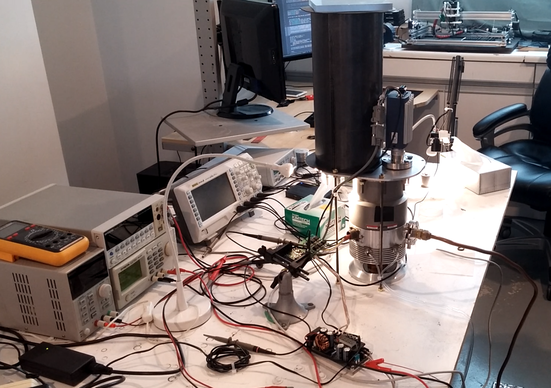
\includegraphics[width=0.5\textwidth]{vacuum}
	}
	\subfloat[]{
	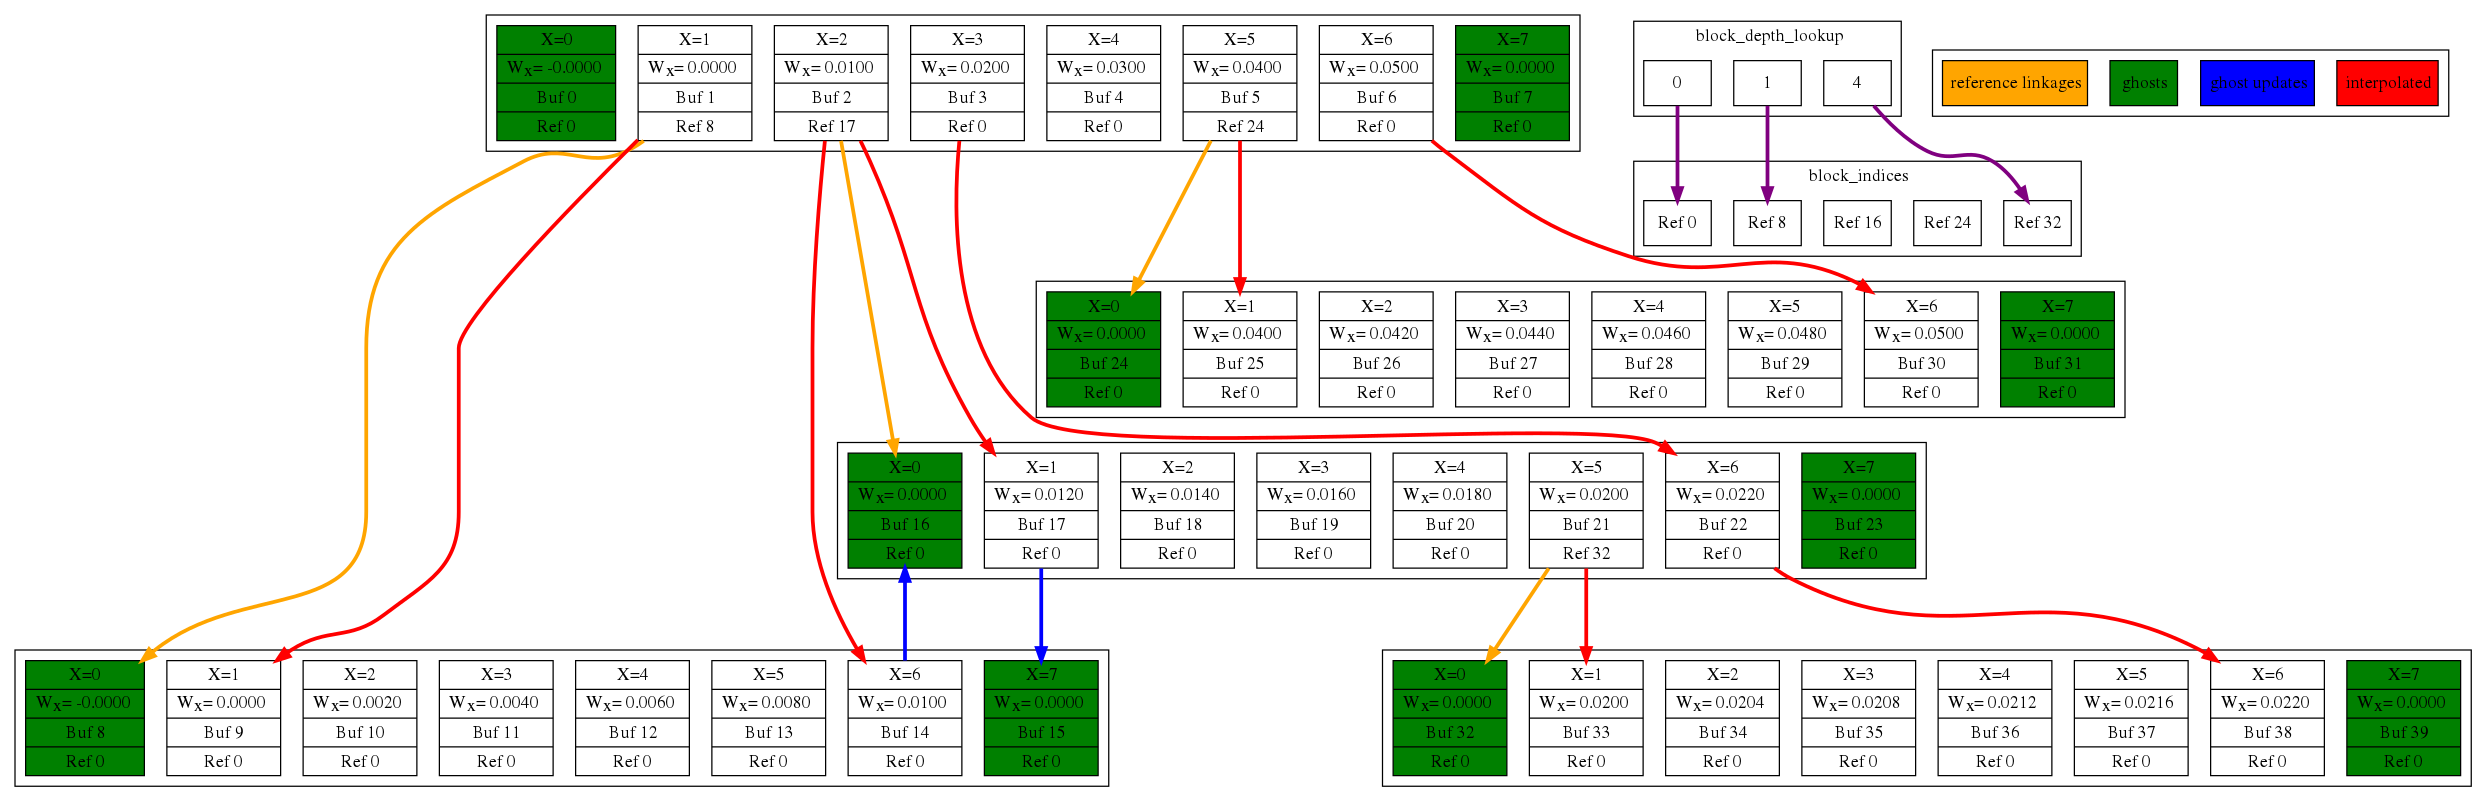
\includegraphics[width=0.5\textwidth]{digraph.png}
	}
	\caption*{Bespoke high vacuum system. GPU-accelerated multigrid data structure and electrostatics solver for particle-in-cell ion beam simulation}
	\hfill
	
\end{figure}



\begin{figure}[H]
	%	\makebox[\textwidth][c]{
	\centering
	\subfloat[]{
		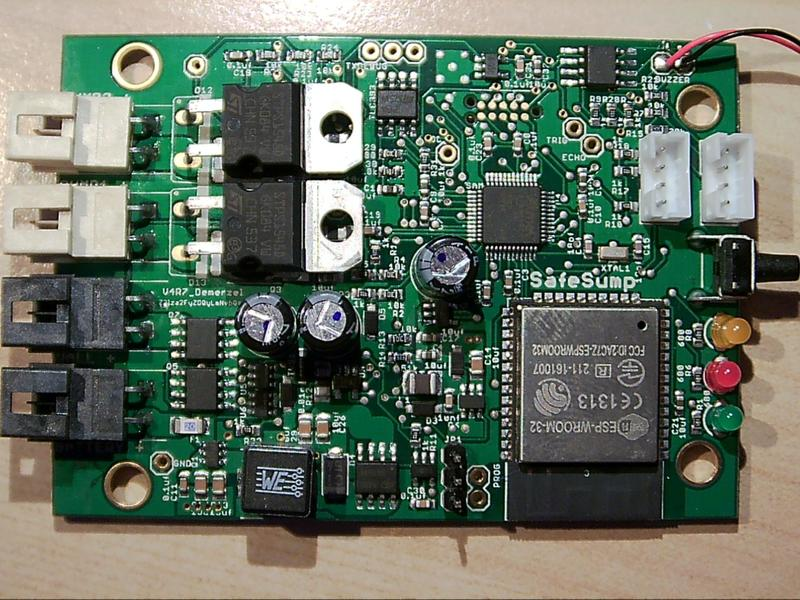
\includegraphics[width=0.4\textwidth]{image1}
		
	}
	\subfloat[]{
		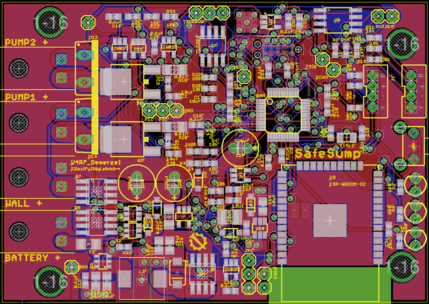
\includegraphics[width=0.4\textwidth]{safesump.png}
		
	}
\caption{Redundant controller with a 120 Mhz Atmel ARM processor, running \ntilde10k lines of high-reliability firmware.}
	\hfill
	
\end{figure}




\end{document}